\documentclass[10pt]{article}
\usepackage[preprint]{tmlr-template/tmlr}
%%%%% NEW MATH DEFINITIONS %%%%%

\usepackage{amsmath,amsfonts,bm}

% Mark sections of captions for referring to divisions of figures
\newcommand{\figleft}{{\em (Left)}}
\newcommand{\figcenter}{{\em (Center)}}
\newcommand{\figright}{{\em (Right)}}
\newcommand{\figtop}{{\em (Top)}}
\newcommand{\figbottom}{{\em (Bottom)}}
\newcommand{\captiona}{{\em (a)}}
\newcommand{\captionb}{{\em (b)}}
\newcommand{\captionc}{{\em (c)}}
\newcommand{\captiond}{{\em (d)}}

% Highlight a newly defined term
\newcommand{\newterm}[1]{{\bf #1}}


% Figure reference, lower-case.
\def\figref#1{figure~\ref{#1}}
% Figure reference, capital. For start of sentence
\def\Figref#1{Figure~\ref{#1}}
\def\twofigref#1#2{figures \ref{#1} and \ref{#2}}
\def\quadfigref#1#2#3#4{figures \ref{#1}, \ref{#2}, \ref{#3} and \ref{#4}}
% Section reference, lower-case.
\def\secref#1{section~\ref{#1}}
% Section reference, capital.
\def\Secref#1{Section~\ref{#1}}
% Reference to two sections.
\def\twosecrefs#1#2{sections \ref{#1} and \ref{#2}}
% Reference to three sections.
\def\secrefs#1#2#3{sections \ref{#1}, \ref{#2} and \ref{#3}}
% Reference to an equation, lower-case.
\def\eqref#1{equation~\ref{#1}}
% Reference to an equation, upper case
\def\Eqref#1{Equation~\ref{#1}}
% A raw reference to an equation---avoid using if possible
\def\plaineqref#1{\ref{#1}}
% Reference to a chapter, lower-case.
\def\chapref#1{chapter~\ref{#1}}
% Reference to an equation, upper case.
\def\Chapref#1{Chapter~\ref{#1}}
% Reference to a range of chapters
\def\rangechapref#1#2{chapters\ref{#1}--\ref{#2}}
% Reference to an algorithm, lower-case.
\def\algref#1{algorithm~\ref{#1}}
% Reference to an algorithm, upper case.
\def\Algref#1{Algorithm~\ref{#1}}
\def\twoalgref#1#2{algorithms \ref{#1} and \ref{#2}}
\def\Twoalgref#1#2{Algorithms \ref{#1} and \ref{#2}}
% Reference to a part, lower case
\def\partref#1{part~\ref{#1}}
% Reference to a part, upper case
\def\Partref#1{Part~\ref{#1}}
\def\twopartref#1#2{parts \ref{#1} and \ref{#2}}

\def\ceil#1{\lceil #1 \rceil}
\def\floor#1{\lfloor #1 \rfloor}
\def\1{\bm{1}}
\newcommand{\train}{\mathcal{D}}
\newcommand{\valid}{\mathcal{D_{\mathrm{valid}}}}
\newcommand{\test}{\mathcal{D_{\mathrm{test}}}}

\def\eps{{\epsilon}}


% Random variables
\def\reta{{\textnormal{$\eta$}}}
\def\ra{{\textnormal{a}}}
\def\rb{{\textnormal{b}}}
\def\rc{{\textnormal{c}}}
\def\rd{{\textnormal{d}}}
\def\re{{\textnormal{e}}}
\def\rf{{\textnormal{f}}}
\def\rg{{\textnormal{g}}}
\def\rh{{\textnormal{h}}}
\def\ri{{\textnormal{i}}}
\def\rj{{\textnormal{j}}}
\def\rk{{\textnormal{k}}}
\def\rl{{\textnormal{l}}}
% rm is already a command, just don't name any random variables m
\def\rn{{\textnormal{n}}}
\def\ro{{\textnormal{o}}}
\def\rp{{\textnormal{p}}}
\def\rq{{\textnormal{q}}}
\def\rr{{\textnormal{r}}}
\def\rs{{\textnormal{s}}}
\def\rt{{\textnormal{t}}}
\def\ru{{\textnormal{u}}}
\def\rv{{\textnormal{v}}}
\def\rw{{\textnormal{w}}}
\def\rx{{\textnormal{x}}}
\def\ry{{\textnormal{y}}}
\def\rz{{\textnormal{z}}}

% Random vectors
\def\rvepsilon{{\mathbf{\epsilon}}}
\def\rvtheta{{\mathbf{\theta}}}
\def\rva{{\mathbf{a}}}
\def\rvb{{\mathbf{b}}}
\def\rvc{{\mathbf{c}}}
\def\rvd{{\mathbf{d}}}
\def\rve{{\mathbf{e}}}
\def\rvf{{\mathbf{f}}}
\def\rvg{{\mathbf{g}}}
\def\rvh{{\mathbf{h}}}
\def\rvu{{\mathbf{i}}}
\def\rvj{{\mathbf{j}}}
\def\rvk{{\mathbf{k}}}
\def\rvl{{\mathbf{l}}}
\def\rvm{{\mathbf{m}}}
\def\rvn{{\mathbf{n}}}
\def\rvo{{\mathbf{o}}}
\def\rvp{{\mathbf{p}}}
\def\rvq{{\mathbf{q}}}
\def\rvr{{\mathbf{r}}}
\def\rvs{{\mathbf{s}}}
\def\rvt{{\mathbf{t}}}
\def\rvu{{\mathbf{u}}}
\def\rvv{{\mathbf{v}}}
\def\rvw{{\mathbf{w}}}
\def\rvx{{\mathbf{x}}}
\def\rvy{{\mathbf{y}}}
\def\rvz{{\mathbf{z}}}

% Elements of random vectors
\def\erva{{\textnormal{a}}}
\def\ervb{{\textnormal{b}}}
\def\ervc{{\textnormal{c}}}
\def\ervd{{\textnormal{d}}}
\def\erve{{\textnormal{e}}}
\def\ervf{{\textnormal{f}}}
\def\ervg{{\textnormal{g}}}
\def\ervh{{\textnormal{h}}}
\def\ervi{{\textnormal{i}}}
\def\ervj{{\textnormal{j}}}
\def\ervk{{\textnormal{k}}}
\def\ervl{{\textnormal{l}}}
\def\ervm{{\textnormal{m}}}
\def\ervn{{\textnormal{n}}}
\def\ervo{{\textnormal{o}}}
\def\ervp{{\textnormal{p}}}
\def\ervq{{\textnormal{q}}}
\def\ervr{{\textnormal{r}}}
\def\ervs{{\textnormal{s}}}
\def\ervt{{\textnormal{t}}}
\def\ervu{{\textnormal{u}}}
\def\ervv{{\textnormal{v}}}
\def\ervw{{\textnormal{w}}}
\def\ervx{{\textnormal{x}}}
\def\ervy{{\textnormal{y}}}
\def\ervz{{\textnormal{z}}}

% Random matrices
\def\rmA{{\mathbf{A}}}
\def\rmB{{\mathbf{B}}}
\def\rmC{{\mathbf{C}}}
\def\rmD{{\mathbf{D}}}
\def\rmE{{\mathbf{E}}}
\def\rmF{{\mathbf{F}}}
\def\rmG{{\mathbf{G}}}
\def\rmH{{\mathbf{H}}}
\def\rmI{{\mathbf{I}}}
\def\rmJ{{\mathbf{J}}}
\def\rmK{{\mathbf{K}}}
\def\rmL{{\mathbf{L}}}
\def\rmM{{\mathbf{M}}}
\def\rmN{{\mathbf{N}}}
\def\rmO{{\mathbf{O}}}
\def\rmP{{\mathbf{P}}}
\def\rmQ{{\mathbf{Q}}}
\def\rmR{{\mathbf{R}}}
\def\rmS{{\mathbf{S}}}
\def\rmT{{\mathbf{T}}}
\def\rmU{{\mathbf{U}}}
\def\rmV{{\mathbf{V}}}
\def\rmW{{\mathbf{W}}}
\def\rmX{{\mathbf{X}}}
\def\rmY{{\mathbf{Y}}}
\def\rmZ{{\mathbf{Z}}}

% Elements of random matrices
\def\ermA{{\textnormal{A}}}
\def\ermB{{\textnormal{B}}}
\def\ermC{{\textnormal{C}}}
\def\ermD{{\textnormal{D}}}
\def\ermE{{\textnormal{E}}}
\def\ermF{{\textnormal{F}}}
\def\ermG{{\textnormal{G}}}
\def\ermH{{\textnormal{H}}}
\def\ermI{{\textnormal{I}}}
\def\ermJ{{\textnormal{J}}}
\def\ermK{{\textnormal{K}}}
\def\ermL{{\textnormal{L}}}
\def\ermM{{\textnormal{M}}}
\def\ermN{{\textnormal{N}}}
\def\ermO{{\textnormal{O}}}
\def\ermP{{\textnormal{P}}}
\def\ermQ{{\textnormal{Q}}}
\def\ermR{{\textnormal{R}}}
\def\ermS{{\textnormal{S}}}
\def\ermT{{\textnormal{T}}}
\def\ermU{{\textnormal{U}}}
\def\ermV{{\textnormal{V}}}
\def\ermW{{\textnormal{W}}}
\def\ermX{{\textnormal{X}}}
\def\ermY{{\textnormal{Y}}}
\def\ermZ{{\textnormal{Z}}}

% Vectors
\def\vzero{{\bm{0}}}
\def\vone{{\bm{1}}}
\def\vmu{{\bm{\mu}}}
\def\vtheta{{\bm{\theta}}}
\def\va{{\bm{a}}}
\def\vb{{\bm{b}}}
\def\vc{{\bm{c}}}
\def\vd{{\bm{d}}}
\def\ve{{\bm{e}}}
\def\vf{{\bm{f}}}
\def\vg{{\bm{g}}}
\def\vh{{\bm{h}}}
\def\vi{{\bm{i}}}
\def\vj{{\bm{j}}}
\def\vk{{\bm{k}}}
\def\vl{{\bm{l}}}
\def\vm{{\bm{m}}}
\def\vn{{\bm{n}}}
\def\vo{{\bm{o}}}
\def\vp{{\bm{p}}}
\def\vq{{\bm{q}}}
\def\vr{{\bm{r}}}
\def\vs{{\bm{s}}}
\def\vt{{\bm{t}}}
\def\vu{{\bm{u}}}
\def\vv{{\bm{v}}}
\def\vw{{\bm{w}}}
\def\vx{{\bm{x}}}
\def\vy{{\bm{y}}}
\def\vz{{\bm{z}}}


% Elements of vectors
\def\evalpha{{\alpha}}
\def\evbeta{{\beta}}
\def\evepsilon{{\epsilon}}
\def\evlambda{{\lambda}}
\def\evomega{{\omega}}
\def\evmu{{\mu}}
\def\evpsi{{\psi}}
\def\evsigma{{\sigma}}
\def\evtheta{{\theta}}
\def\eva{{a}}
\def\evb{{b}}
\def\evc{{c}}
\def\evd{{d}}
\def\eve{{e}}
\def\evf{{f}}
\def\evg{{g}}
\def\evh{{h}}
\def\evi{{i}}
\def\evj{{j}}
\def\evk{{k}}
\def\evl{{l}}
\def\evm{{m}}
\def\evn{{n}}
\def\evo{{o}}
\def\evp{{p}}
\def\evq{{q}}
\def\evr{{r}}
\def\evs{{s}}
\def\evt{{t}}
\def\evu{{u}}
\def\evv{{v}}
\def\evw{{w}}
\def\evx{{x}}
\def\evy{{y}}
\def\evz{{z}}

% Matrix
\def\mA{{\bm{A}}}
\def\mB{{\bm{B}}}
\def\mC{{\bm{C}}}
\def\mD{{\bm{D}}}
\def\mE{{\bm{E}}}
\def\mF{{\bm{F}}}
\def\mG{{\bm{G}}}
\def\mH{{\bm{H}}}
\def\mI{{\bm{I}}}
\def\mJ{{\bm{J}}}
\def\mK{{\bm{K}}}
\def\mL{{\bm{L}}}
\def\mM{{\bm{M}}}
\def\mN{{\bm{N}}}
\def\mO{{\bm{O}}}
\def\mP{{\bm{P}}}
\def\mQ{{\bm{Q}}}
\def\mR{{\bm{R}}}
\def\mS{{\bm{S}}}
\def\mT{{\bm{T}}}
\def\mU{{\bm{U}}}
\def\mV{{\bm{V}}}
\def\mW{{\bm{W}}}
\def\mX{{\bm{X}}}
\def\mY{{\bm{Y}}}
\def\mZ{{\bm{Z}}}
\def\mBeta{{\bm{\beta}}}
\def\mPhi{{\bm{\Phi}}}
\def\mLambda{{\bm{\Lambda}}}
\def\mSigma{{\bm{\Sigma}}}

% Tensor
\DeclareMathAlphabet{\mathsfit}{\encodingdefault}{\sfdefault}{m}{sl}
\SetMathAlphabet{\mathsfit}{bold}{\encodingdefault}{\sfdefault}{bx}{n}
\newcommand{\tens}[1]{\bm{\mathsfit{#1}}}
\def\tA{{\tens{A}}}
\def\tB{{\tens{B}}}
\def\tC{{\tens{C}}}
\def\tD{{\tens{D}}}
\def\tE{{\tens{E}}}
\def\tF{{\tens{F}}}
\def\tG{{\tens{G}}}
\def\tH{{\tens{H}}}
\def\tI{{\tens{I}}}
\def\tJ{{\tens{J}}}
\def\tK{{\tens{K}}}
\def\tL{{\tens{L}}}
\def\tM{{\tens{M}}}
\def\tN{{\tens{N}}}
\def\tO{{\tens{O}}}
\def\tP{{\tens{P}}}
\def\tQ{{\tens{Q}}}
\def\tR{{\tens{R}}}
\def\tS{{\tens{S}}}
\def\tT{{\tens{T}}}
\def\tU{{\tens{U}}}
\def\tV{{\tens{V}}}
\def\tW{{\tens{W}}}
\def\tX{{\tens{X}}}
\def\tY{{\tens{Y}}}
\def\tZ{{\tens{Z}}}


% Graph
\def\gA{{\mathcal{A}}}
\def\gB{{\mathcal{B}}}
\def\gC{{\mathcal{C}}}
\def\gD{{\mathcal{D}}}
\def\gE{{\mathcal{E}}}
\def\gF{{\mathcal{F}}}
\def\gG{{\mathcal{G}}}
\def\gH{{\mathcal{H}}}
\def\gI{{\mathcal{I}}}
\def\gJ{{\mathcal{J}}}
\def\gK{{\mathcal{K}}}
\def\gL{{\mathcal{L}}}
\def\gM{{\mathcal{M}}}
\def\gN{{\mathcal{N}}}
\def\gO{{\mathcal{O}}}
\def\gP{{\mathcal{P}}}
\def\gQ{{\mathcal{Q}}}
\def\gR{{\mathcal{R}}}
\def\gS{{\mathcal{S}}}
\def\gT{{\mathcal{T}}}
\def\gU{{\mathcal{U}}}
\def\gV{{\mathcal{V}}}
\def\gW{{\mathcal{W}}}
\def\gX{{\mathcal{X}}}
\def\gY{{\mathcal{Y}}}
\def\gZ{{\mathcal{Z}}}

% Sets
\def\sA{{\mathbb{A}}}
\def\sB{{\mathbb{B}}}
\def\sC{{\mathbb{C}}}
\def\sD{{\mathbb{D}}}
% Don't use a set called E, because this would be the same as our symbol
% for expectation.
\def\sF{{\mathbb{F}}}
\def\sG{{\mathbb{G}}}
\def\sH{{\mathbb{H}}}
\def\sI{{\mathbb{I}}}
\def\sJ{{\mathbb{J}}}
\def\sK{{\mathbb{K}}}
\def\sL{{\mathbb{L}}}
\def\sM{{\mathbb{M}}}
\def\sN{{\mathbb{N}}}
\def\sO{{\mathbb{O}}}
\def\sP{{\mathbb{P}}}
\def\sQ{{\mathbb{Q}}}
\def\sR{{\mathbb{R}}}
\def\sS{{\mathbb{S}}}
\def\sT{{\mathbb{T}}}
\def\sU{{\mathbb{U}}}
\def\sV{{\mathbb{V}}}
\def\sW{{\mathbb{W}}}
\def\sX{{\mathbb{X}}}
\def\sY{{\mathbb{Y}}}
\def\sZ{{\mathbb{Z}}}

% Entries of a matrix
\def\emLambda{{\Lambda}}
\def\emA{{A}}
\def\emB{{B}}
\def\emC{{C}}
\def\emD{{D}}
\def\emE{{E}}
\def\emF{{F}}
\def\emG{{G}}
\def\emH{{H}}
\def\emI{{I}}
\def\emJ{{J}}
\def\emK{{K}}
\def\emL{{L}}
\def\emM{{M}}
\def\emN{{N}}
\def\emO{{O}}
\def\emP{{P}}
\def\emQ{{Q}}
\def\emR{{R}}
\def\emS{{S}}
\def\emT{{T}}
\def\emU{{U}}
\def\emV{{V}}
\def\emW{{W}}
\def\emX{{X}}
\def\emY{{Y}}
\def\emZ{{Z}}
\def\emSigma{{\Sigma}}

% entries of a tensor
% Same font as tensor, without \bm wrapper
\newcommand{\etens}[1]{\mathsfit{#1}}
\def\etLambda{{\etens{\Lambda}}}
\def\etA{{\etens{A}}}
\def\etB{{\etens{B}}}
\def\etC{{\etens{C}}}
\def\etD{{\etens{D}}}
\def\etE{{\etens{E}}}
\def\etF{{\etens{F}}}
\def\etG{{\etens{G}}}
\def\etH{{\etens{H}}}
\def\etI{{\etens{I}}}
\def\etJ{{\etens{J}}}
\def\etK{{\etens{K}}}
\def\etL{{\etens{L}}}
\def\etM{{\etens{M}}}
\def\etN{{\etens{N}}}
\def\etO{{\etens{O}}}
\def\etP{{\etens{P}}}
\def\etQ{{\etens{Q}}}
\def\etR{{\etens{R}}}
\def\etS{{\etens{S}}}
\def\etT{{\etens{T}}}
\def\etU{{\etens{U}}}
\def\etV{{\etens{V}}}
\def\etW{{\etens{W}}}
\def\etX{{\etens{X}}}
\def\etY{{\etens{Y}}}
\def\etZ{{\etens{Z}}}

% The true underlying data generating distribution
\newcommand{\pdata}{p_{\rm{data}}}
% The empirical distribution defined by the training set
\newcommand{\ptrain}{\hat{p}_{\rm{data}}}
\newcommand{\Ptrain}{\hat{P}_{\rm{data}}}
% The model distribution
\newcommand{\pmodel}{p_{\rm{model}}}
\newcommand{\Pmodel}{P_{\rm{model}}}
\newcommand{\ptildemodel}{\tilde{p}_{\rm{model}}}
% Stochastic autoencoder distributions
\newcommand{\pencode}{p_{\rm{encoder}}}
\newcommand{\pdecode}{p_{\rm{decoder}}}
\newcommand{\precons}{p_{\rm{reconstruct}}}

\newcommand{\laplace}{\mathrm{Laplace}} % Laplace distribution

\newcommand{\E}{\mathbb{E}}
\newcommand{\Ls}{\mathcal{L}}
\newcommand{\R}{\mathbb{R}}
\newcommand{\emp}{\tilde{p}}
\newcommand{\lr}{\alpha}
\newcommand{\reg}{\lambda}
\newcommand{\rect}{\mathrm{rectifier}}
\newcommand{\softmax}{\mathrm{softmax}}
\newcommand{\sigmoid}{\sigma}
\newcommand{\softplus}{\zeta}
\newcommand{\KL}{D_{\mathrm{KL}}}
\newcommand{\Var}{\mathrm{Var}}
\newcommand{\standarderror}{\mathrm{SE}}
\newcommand{\Cov}{\mathrm{Cov}}
% Wolfram Mathworld says $L^2$ is for function spaces and $\ell^2$ is for vectors
% But then they seem to use $L^2$ for vectors throughout the site, and so does
% wikipedia.
\newcommand{\normlzero}{L^0}
\newcommand{\normlone}{L^1}
\newcommand{\normltwo}{L^2}
\newcommand{\normlp}{L^p}
\newcommand{\normmax}{L^\infty}

\newcommand{\parents}{Pa} % See usage in notation.tex. Chosen to match Daphne's book.

\DeclareMathOperator*{\argmax}{arg\,max}
\DeclareMathOperator*{\argmin}{arg\,min}

\DeclareMathOperator{\sign}{sign}
\DeclareMathOperator{\Tr}{Tr}
\let\ab\allowbreak

\usepackage{amssymb,graphicx,mathtools}
\usepackage[OT1]{fontenc}
\usepackage{hyperref}
\usepackage{url}
\title{Two Mechanisms of Model-Wise Double Descent:\\Frozen Kernels and Feature Learning}
\author{\name Viktor Vesel\'{y} \email v.vesely@student.rug.nl \\
\addr University of Groningen}

\begin{document}
\maketitle
\begin{abstract}
We propose that model-wise double descent can arise from two distinct, potentially coexisting mechanisms. Frozen-kernel double descent (FKDD) results from fitting residual components in weak kernel modes whose amplification harms generalization. Feature-learning double descent (FLDD) instead involves changes in representation that facilitate fitting label noise and transfer harmfully to unseen data. Our central claim is that these are separable sources of non-monotonic generalization across model size, rather than interchangeable explanations of a single peak. We propose a sample-level mechanism for FLDD and two ablations: freezing the entire Jacobian, and selectively blocking feature updates from samples that help noise fitting while retaining their training losses. This preliminary note introduces the distinction, the proposed mechanism, and the experiments designed to establish their connection.
\end{abstract}

\section{Claim and relation to existing work}
\textbf{Model-wise double descent need not have a single mechanism.} At a fixed training budget, validation loss can decrease, increase, and decrease again as width grows. We distinguish a \emph{frozen-kernel} source of this behavior from a \emph{feature-learning} source. Both may operate in the same task and architecture family, at different widths or training times, and potentially overlap within the same width sweep. Their different width and time scales explain how an early feature-learning peak and a later frozen-kernel peak can arise in the same model family.

Two strands of work motivate this distinction. Fixed-feature analyses explain double descent without representation learning: Bach~\cite{bach2023highdimensionalanalysisdoubledescent} studies linear regression with random projections. Learned-feature explanations instead emphasize noise fitting and changes in representation; Gu et al.~\cite{gu2024unravelingenigmadoubledescent} connect double descent to the learned feature space and separation of signal from noise. These strands are not a strict partition: Singh et al.~\cite{singh2022phenomenologydoubledescentfinitewidth} analyze finite-width networks through influence functions and Hessian spectra, while Litman and Guo~\cite{litman2026theorygeneralizationdeeplearning} develop a signal--noise kernel perspective that explicitly allows feature learning.

Han et al.~\cite{pmlr-v267-han25c} provide a particularly close precursor: their analysis describes learning signal from clean samples followed by memorization of noise and degraded generalization. Our proposed contribution is more specific than the observation that feature learning can help memorize noise: \emph{to distinguish FLDD from FKDD as potentially coexisting model-wise phenomena, and to test FLDD by intervening on the samples responsible for noise-helpful feature changes}. This connects the dynamics of noise memorization to the width dependence of generalization and separates it from the frozen-kernel mechanism.

\section{Two double-descent mechanisms}
Let $\sS$ be the training set, $\sN\subset\sS$ its fixed label-corrupted subset, and $\sQ$ a clean validation set. For a sample set $\sA$, let $\vf_{\sA}$ concatenate its model outputs and define
\begin{equation}
 \mJ_{\sA}=\nabla_{\vtheta}\vf_{\sA},\qquad
 \vg_{\sA}=\nabla_{\vf_{\sA}}\mathcal L_{\sA},\qquad
 \mK_{\sA\sB}=\mJ_{\sA}\mJ_{\sB}^{\top}.
\end{equation}
For a batch $\sB$, SGD takes $\vtheta^+=\vtheta-\alpha\vp_{\sB}$, where $\vp_{\sB}=\mJ_{\sB}^{\top}\vg_{\sB}=\sum_{i\in\sB}\vp_i$ and $\vp_i$ is sample $i$'s contribution to the parameter gradient. All sample contributions retain the batch loss normalization.

\paragraph{FKDD: amplification through weak modes.}
With a fixed Jacobian, consider squared loss and an eigenpair $\mK_{\sS\sS}\vu_j=\lambda_j\vu_j$, $\lambda_j>0$. Under gradient flow, the contribution to validation predictions from the initial residual $\vr_0=\vy_{\sS}-\vf_{\sS}(0)$ is
\begin{equation}
 \Delta\vf_{\sQ}^{(j)}(t)
 =\mK_{\sQ\sS}\vu_j
 \frac{1-e^{-\lambda_j t}}{\lambda_j}
 \vu_j^\top\vr_0.
 \label{eq:fk}
\end{equation}
Time absorbs the loss normalization. FKDD arises when weak modes carry residual error and their eventual fitting transfers harmfully to validation. These modes require large coefficients and long training times. Their width-dependent amplification produces a peak that can emerge much later than FLDD.

\paragraph{FLDD: feature changes that facilitate harmful noise fitting.}
We propose that some training samples create features that make noisy targets easier to fit. At widths with sufficient capacity to fit the noise, this accelerates memorization and raises validation loss. At greater width, a representation that better separates signal and noise can reduce harmful transfer, producing the second descent. The mechanism combines three conditions: creation of noise-helpful features, sufficient capacity to fit noise, and harmful transfer of the fitted noise to validation. The samples creating these features can include both clean and corrupted samples.

To identify their contribution, follow one fixed SGD direction, $\vtheta(\tau)=\vtheta-\tau\vp_{\sB}$. For the corrupted samples in the batch, write $\sN_{\sB}=\sN\cap\sB$. At the start of the step,
\begin{align}
 \mH_{\sN_{\sB}}^{\mathrm{feat}}
 &=\sum_a(\vg_{\sN_{\sB}})_a\nabla_{\vtheta}^2(\vf_{\sN_{\sB}})_a,
 \\[-2pt]
 \frac{d^2\mathcal L_{\sN_{\sB}}}{d\tau^2}
 &=\underbrace{\vp_{\sB}^{\top}\mJ_{\sN_{\sB}}^{\top}
 \bigl(\nabla_{\vf_{\sN_{\sB}}}^2\mathcal L_{\sN_{\sB}}\bigr)
 \mJ_{\sN_{\sB}}\vp_{\sB}}_{\text{Loss curvature}}
 +\underbrace{\vp_{\sB}^{\top}\mH_{\sN_{\sB}}^{\mathrm{feat}}\vp_{\sB}}_{\text{Feature-learning curvature}}.
 \label{eq:curvature}
\end{align}
The feature-learning term is zero for a frozen-Jacobian model. To express its sample-level meaning, define the instantaneous ease of noise fitting as $\ell_{\sN_{\sB}}=\vg_{\sN_{\sB}}^\top\mJ_{\sN_{\sB}}\vp_{\sB}$. The change in this quantity caused by changing the Jacobian along sample $i$'s update direction is
\begin{equation}
 D_{-\vp_i}^{\mathrm{feat}}\ell_{\sN_{\sB}}
 =-\vg_{\sN_{\sB}}^\top
 D_{\vp_i}\mJ_{\sN_{\sB}}
 \vp_{\sB}
 =-\vp_i^\top\mH_{\sN_{\sB}}^{\mathrm{feat}}\vp_{\sB}.
 \label{eq:ease}
\end{equation}
Here $D^{\mathrm{feat}}$ holds the output gradient and the batch update direction fixed, isolating the change in features. Thus
\begin{equation}
 h_i=-\frac{\alpha^2}{2}\vp_i^\top\mH_{\sN_{\sB}}^{\mathrm{feat}}\vp_{\sB},
 \qquad
 \sum_{i\in\sB}h_i=
 -\frac{\alpha^2}{2}\vp_{\sB}^\top\mH_{\sN_{\sB}}^{\mathrm{feat}}\vp_{\sB}.
 \label{eq:help}
\end{equation}
Positive $h_i$ means that sample $i$'s update locally changes features in a direction that facilitates noise fitting. The factor $\alpha^2/2$ puts this contribution on the scale of the second-order loss change. We aggregate these contributions along training, using subdivided update paths to capture feature changes within a step. Harmful transfer is measured separately through the first-order validation effect of noise updates, $-\alpha\vg_{\sQ}^\top\mJ_{\sQ}\mJ_{\sN_{\sB}}^\top\vg_{\sN_{\sB}}>0$.

\begin{figure}[t]
 \centering
 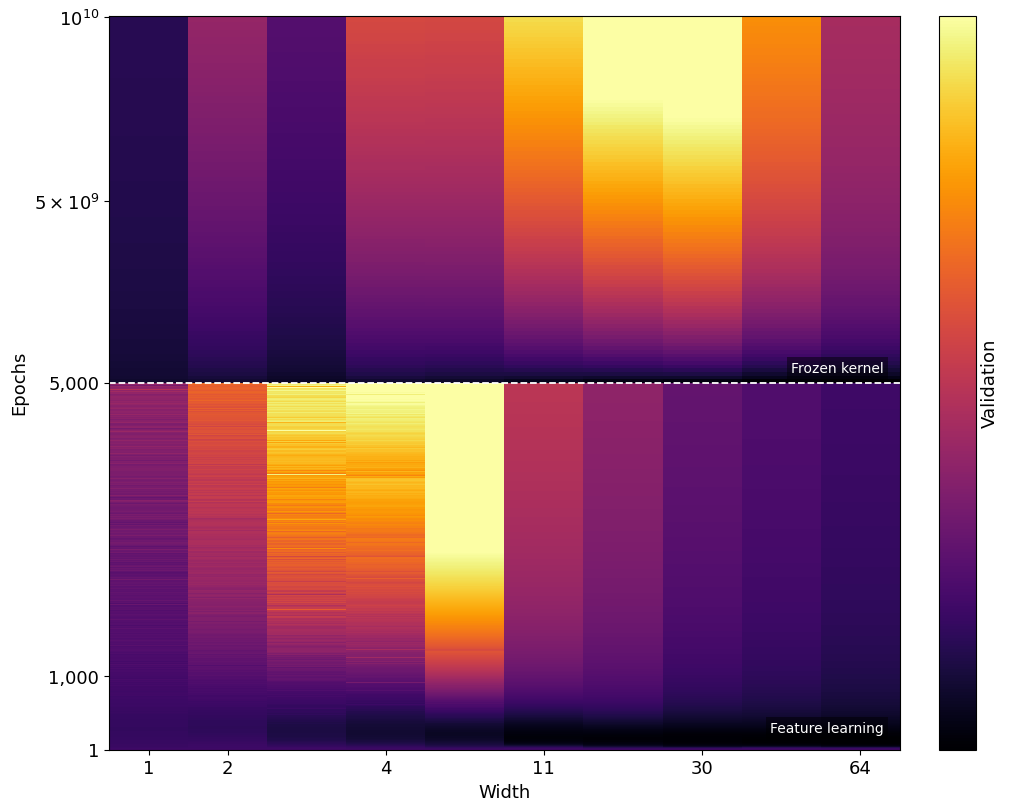
\includegraphics[width=0.57\linewidth]{../showcase_of_double_dd.png}
 \caption{Two model-wise double descents at different widths and training times. The lower panel shows the early feature-learning peak; the upper panel shows the later frozen-kernel peak. The two regimes are displayed on a broken time axis. Colors indicate validation loss.}
 \label{fig:motivation}
\end{figure}

\section{Two proposed ablations}
\paragraph{1. Identify the distinction between FLDD and FKDD.}
The first ablation tests whether the early and late double descents have different origins. Starting from the same initialization at each width, compare the feature-learning model with its frozen-Jacobian counterpart:
\begin{equation}
 \bar f(\vx;\vw)
 =f_{\vtheta_0}(\vx)
 +\mJ_{\vtheta_0}(\vx)\vw,
 \qquad \vw_0=\vzero.
\end{equation}
Keep the task, corrupted labels, batch order, learning rate, and trainable parameter count matched within each width. At the feature-learning training budget, we predict an FLDD peak in the feature-learning model and its disappearance under freezing. Continuing frozen-kernel training then reveals the second, later DD as slow modes are fitted. The contrast identifies two distinct double descents: one depends on feature evolution, while the other arises with fixed features. Matched-loss training provides the direct comparison; long-time squared-loss kernel predictions resolve the slow-mode behavior analytically.

\paragraph{2. Test the proposed FLDD mechanism.}
The second ablation tests whether the FLDD peak is driven by samples creating features that help fit noise. Rank samples by their accumulated positive $h_i$ contribution at the FLDD peak width, averaged over seeds. Select a prescribed fraction of the positive contribution and reuse the same sample mask across widths. Retrain while disabling those samples' feature-learning updates but retaining their losses and their ability to learn through a fixed-feature pathway. The tangent implementation routes selected updates through the initial Jacobian; the mixed implementation blocks their hidden-layer gradients while retaining readout learning.

The mechanism predicts that this targeted intervention reduces the FLDD peak while the selected samples can still be fitted. Equal-count random blocking tests the specificity of the identified feature creators; removing the same samples' learning contribution provides a comparison with excluding them altogether. Selected-sample training losses and extended training establish whether peak suppression persists when those samples are fitted. Together, the two ablations separate the existence of two DD mechanisms from the proposed explanation of FLDD.

\paragraph{Research scope.}
This preliminary note proposes the distinction and mechanism for noisy-label MNIST and CIFAR-10 width sweeps. The accompanying ablations are designed to establish how feature-mediated noise fitting and slow frozen-kernel modes produce distinct, potentially coexisting model-wise double descents.

\bibliography{tmlr-template/tmlr}
\bibliographystyle{tmlr-template/tmlr}
\end{document}
